\chapter{Valutazioni sperimentali}\label{cha:valutazioni_sperimentali}
Conclusa la fase di definizione algoritmica e di modellazione teorica della soluzione, questo capitolo si concentra sull'analisi sperimentale dell'approccio proposto.
L'obbiettivo di tale analisi è sia quello di verificare l'efficienza computazionale del sistema in termini di tempi di risposta e scalabilità; sia quello di valutare l'efficacia e la robustezza dell'algoritmo nella ricerca di soluzioni di alta qualità al variare della complessità del problema.

% 4.1
% Revisione Ready
% Grammatica Ready
% Citazioni Ready

\section{Configurazione e ambiente di test}\label{sec:configurazione_e_ambiente_di_test}

Gli esperimenti che seguiranno all'interno di questo capitolo sono stati condotti all'interno dello stesso ambiente e sulla stessa macchina, in modo da poter garantire omogeneità tra i vari casi di test.
Inoltre, per garantire confrontabilità e ripetitività dei test eseguiti procedo a specificare le caratteristiche tecniche delle componenti da me utilizzate.
\begin{itemize}
    \item \textbf{Hardware}: i test sono stati effettuati nella loro interezza su un laptop con processore AMD Ryzen 7 5700U e con 8 GB di memoria RAM.
    Poiché l'algoritmo proposto non implementa logiche di parallelizzazione, le prestazioni riportate si riferiscono esclusivamente all'esecuzione del processo in modalità \textit{single-thread}.
    \item \textbf{Software}: il programma è stato sviluppato interamente in Python (v 3.14), sfruttando delle librerie di supporto quali \texttt{hypergraphx}~\cite{lotito2023} per la gestione degli ipergrafi temporali e \texttt{time} per la misurazione dei tempi di esecuzione.
\end{itemize}

% 4.2
% Revisione Ready
% Grammatica Ready
% Citazioni Ready

\section{Varianti degli algoritmi analizzati}\label{sec:varianti_degli_algoritmi_analizzati}

Per analizzare l'impatto che ogni componente della soluzione implementata ha sul sistema intero abbiamo deciso di testare diverse versioni dello stesso algoritmo, variando per ognuna di esse una scelta progettuale, in modo da valutarne l'importanza relativa.
Questo approccio permette di isolare il contributo di una scelta progettuale alla volta, evitando che le differenze osservate tra le configurazioni siano attribuibili a più fattori sovrapposti.
Sono state definite quattro varianti diverse di algoritmi, riassunte di seguito:
\begin{itemize}
    \item \textbf{Iterative Greedy}: questo algoritmo consiste in una versione nella quale viene applicato un algoritmo greedy in maniera naïve, che ricalcola da capo l'intero Hitting Set ad ogni spostamento della finestra temporale.
    \item \textbf{Sliding different Greedy}: questo algoritmo rappresenta una variazione di quello presentato nella soluzione proposta (si veda il Capitolo~\ref{sec:soluzione_proposta}); in particolare vengono modificate le funzioni \texttt{GreedyHittingSet} e \texttt{ReuseGreedyHittingSet}, applicando una tipologia diversa di algoritmo greedy per valutare il contributo di tale algoritmo sia dal punto di vista del tempo di esecuzione che della dimensione media dell'Hitting Set risultante.
    \item \textbf{Sliding New Nodes}: questo algoritmo rappresenta una variazione di quello presentato nella soluzione proposta (si veda il Capitolo~\ref{sec:soluzione_proposta}); in particolare viene modificata la gestione dei pesi all'interno della funzione \texttt{ReuseGreedyHittingSet}, i pesi vengono invertiti portando l'algoritmo a preferire la scelta di nodi senza uno storico all'interno degli Hitting Set precedenti.
    \item \textbf{Sliding Reuse}: questo algoritmo coincide con quello presentato nella soluzione proposta (si veda il Capitolo~\ref{sec:soluzione_proposta}).
\end{itemize}

\subsection*{Algoritmi greedy utilizzati}

Nel corso della descrizione della soluzione proposta (si veda il Capitolo~\ref{sec:soluzione_proposta}) e della precedente esposizione delle varianti algoritmiche utilizzate nella fase di test, sono stati citati più volte alcuni algoritmi risolutivi greedy, senza però aver approfondito i rispettivi dettagli implementativi.
Come discusso nella sezione delle soluzioni euristiche per il problema dell'Hitting Set analizzato in ambito statico (si veda la Sezione~\ref{sec:minimum_hitting_set_in_ambito_statico}), gli algoritmi greedy per il Minimum Hitting Set possono essere classificati in euristiche \emph{vertex-oriented}, che privilegiano il contributo globale alla copertura, ed euristiche \emph{hyperedge-oriented}, che operano invece una scelta locale basata sull'iperarco analizzato~\cite{gainer2017}.
Gli algoritmi greedy utilizzati all'interno di questo lavoro fanno parte della famiglia delle euristiche \emph{hyperedge-oriented}, più precisamente sono state utilizzare due varianti distinte:
\begin{itemize}
    \item \textbf{Nodo di cardinalità massima in iperarco minimo}: variante utilizzata nelle versioni \texttt{Iterative Greedy}, \texttt{Sliding New Nodes} e \texttt{Sliding Reuse}.
    Consiste nella pratica di selezionare come nuovo nodo dell'Hitting Set il nodo di cardinalità massima che fa parte dell'iperarco non coperto di cardinalità minima.
    La versione della funzione \texttt{ReuseGreedyHittingSet} si differenzia dalla funzione \texttt{GreedyHittingSet} in quanto in caso di più nodi con la stessa cardinalità massima si seleziona quello con uno storico all'interno degli Hitting Set precedenti, eccezione fatta per la versione \texttt{Sliding New Nodes} che come spiegato in precedenza inverte la scelta di priorità.
    \item \textbf{Nodo di cardinalità massima in iperarco randomico}: variante utilizzata nella versione \texttt{Sliding different Greedy}.
    Consiste nella pratica di selezionare come nuovo nodo dell'Hitting Set il nodo di cardinalità massima che fa parte di un iperarco non coperto selezionato in maniera randomica.
    La versione della funzione \texttt{ReuseGreedyHittingSet} si differenzia dalla funzione \texttt{GreedyHittingSet} in quanto in caso di più nodi con la stessa cardinalità massima si seleziona quello con uno storico all'interno degli Hitting Set precedenti.
\end{itemize}

% 4.3
% Revisione Ready
% Grammatica Ready
% Citazioni Ready

\section{Istanze di benchmark e caratterizzazione dei dati}\label{sec:istanze_di_benchmark_e_caratterizzazione_dei_dati}

Per valutare le prestazioni degli algoritmi presentati nel capitolo precedente è necessario specificare anche l'insieme dei dataset sui quali sono stati fatti girare gli algoritmi.
Per valutare al meglio la robustezza e la capacità di generalizzazione degli algoritmi proposti, i test sono stati condotti su un insieme di quattro istanze diversificate.
Per generalizzare il più possibile sono stati presi in considerazione dataset differenti in dimensione e distribuzione temporale, l'unico elemento comune è che tutte le istanze sono state tratte da dati reali ampiamente utilizzati nella letteratura degli ipergrafi temporali~\cite{lotito2023}.
Le caratteristiche strutturali ed evolutive delle istanze selezionate sono riassunte nella seguente Tabella ~\ref{tab:caratteristiche_dataset}.
\begin{table}[htbp]
\centering
\caption{Proprietà strutturali delle istanze di benchmark utilizzate.}
\label{tab:caratteristiche_dataset}
\begin{tabular}{lcccc}
\hline
\textbf{ID Dataset} & \textbf{Nodi ($|V|$)} & \textbf{Iperarchi ($|E|$)} & \textbf{Iperarchi unici ($|E|$)} \\ \hline
Contacts high school& $3\cdot 10^3$         & $1.7\cdot 10^5$             & $7.8\cdot 10^3$     \\
Coauth history      & $1\cdot 10^6$         & $1.8\cdot 10^6$             & $9\cdot 10^5$       \\
Email Enron         & $8.4\cdot 10^4$       & $2.4\cdot 10^5$             & $1.1\cdot 10^5$     \\
Crypto bitcoin      & $2.5\cdot 10^6$       & $1.5\cdot 10^6$             & $1.3\cdot 10^6$     \\ \hline
\end{tabular}
\end{table}

\subsection*{Analisi delle distribuzioni strutturali}
Un fattore cruciale per determinare l'efficacia della soluzione basata sulla finestra temporale a scorrimento è la distribuzione intrinseca dei dati.
La seguente figura (si veda Figura~\ref{fig:distribuzione_dataset}) mostra la distribuzione che definisce il numero di iperarchi che arrivano al tempo $\tau_k$ per le istanze principali.
% Esempio di inserimento delle tue immagini affiancate per risparmiare spazio
\begin{figure}[htbp]
    \centering
    \begin{minipage}{0.48\textwidth}
        \centering
        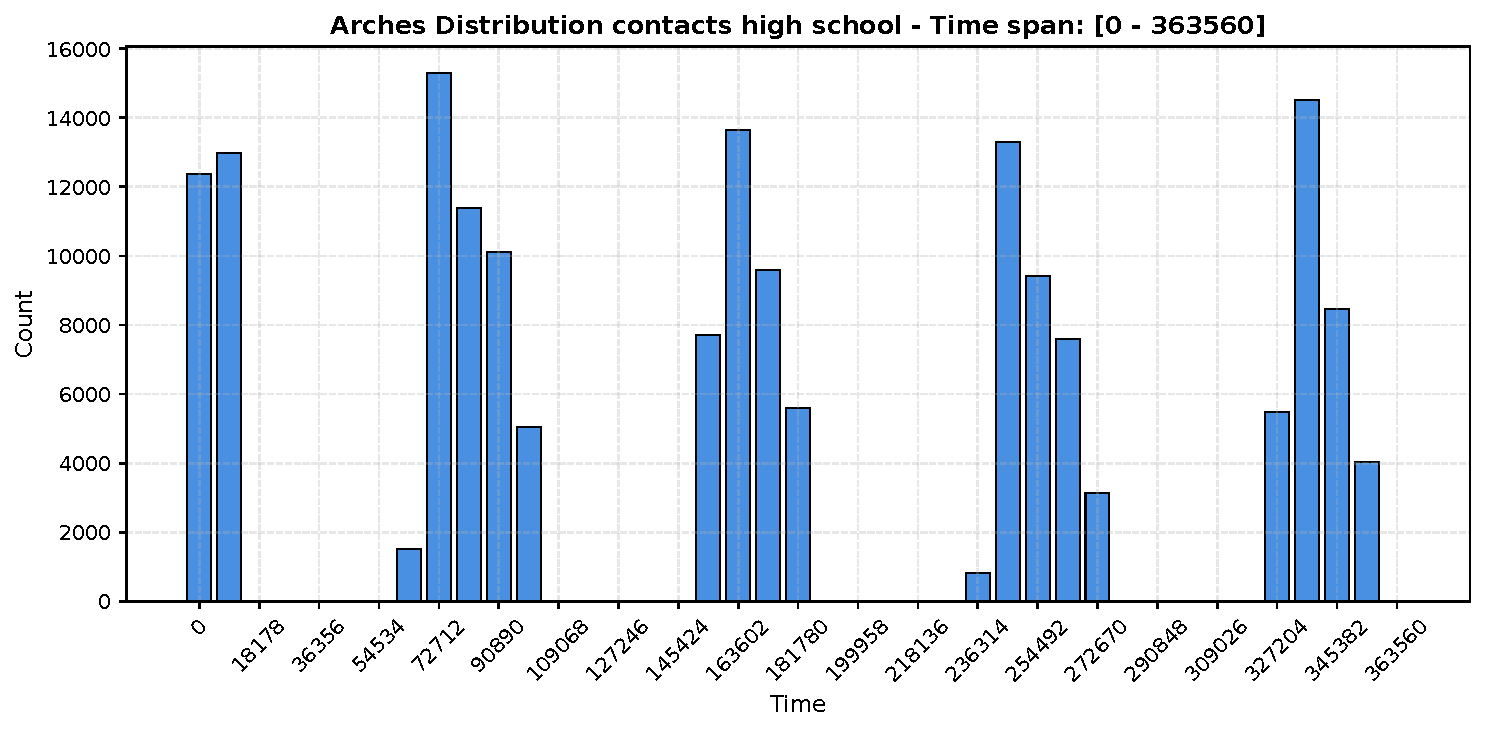
\includegraphics[width=\textwidth]{Immagini/arches_distribution_graph/contacts_high_school.pdf}
        \vspace{-9mm}
        \caption*{(a) Dataset Contacts high school}
    \end{minipage}
    \hfill
    \begin{minipage}{0.48\textwidth}
        \centering
        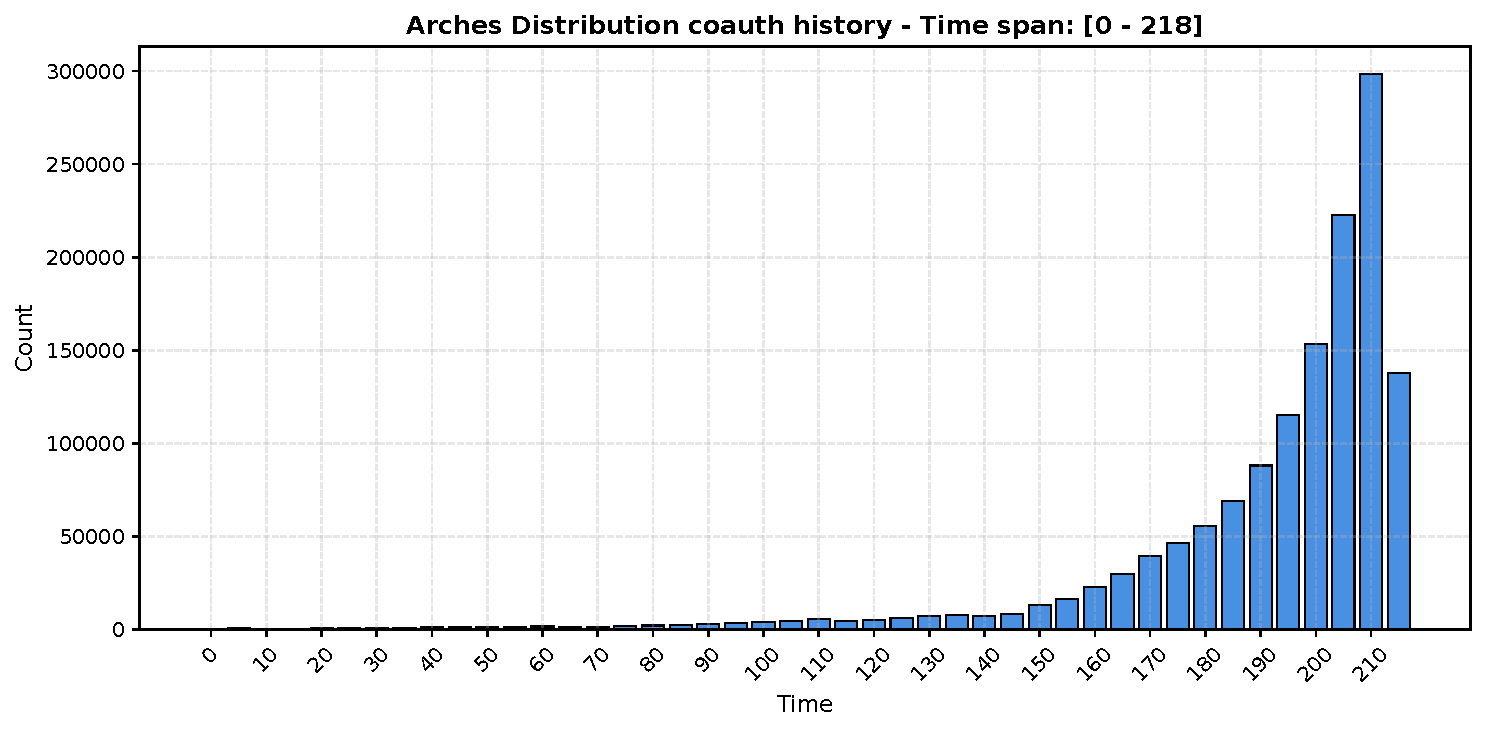
\includegraphics[width=\textwidth]{Immagini/arches_distribution_graph/coauth_history.pdf}
        \vspace{-9mm}
        \caption*{(b) Dataset Coauth history}
    \end{minipage}
    \centering
    \begin{minipage}{0.48\textwidth}
        \centering
        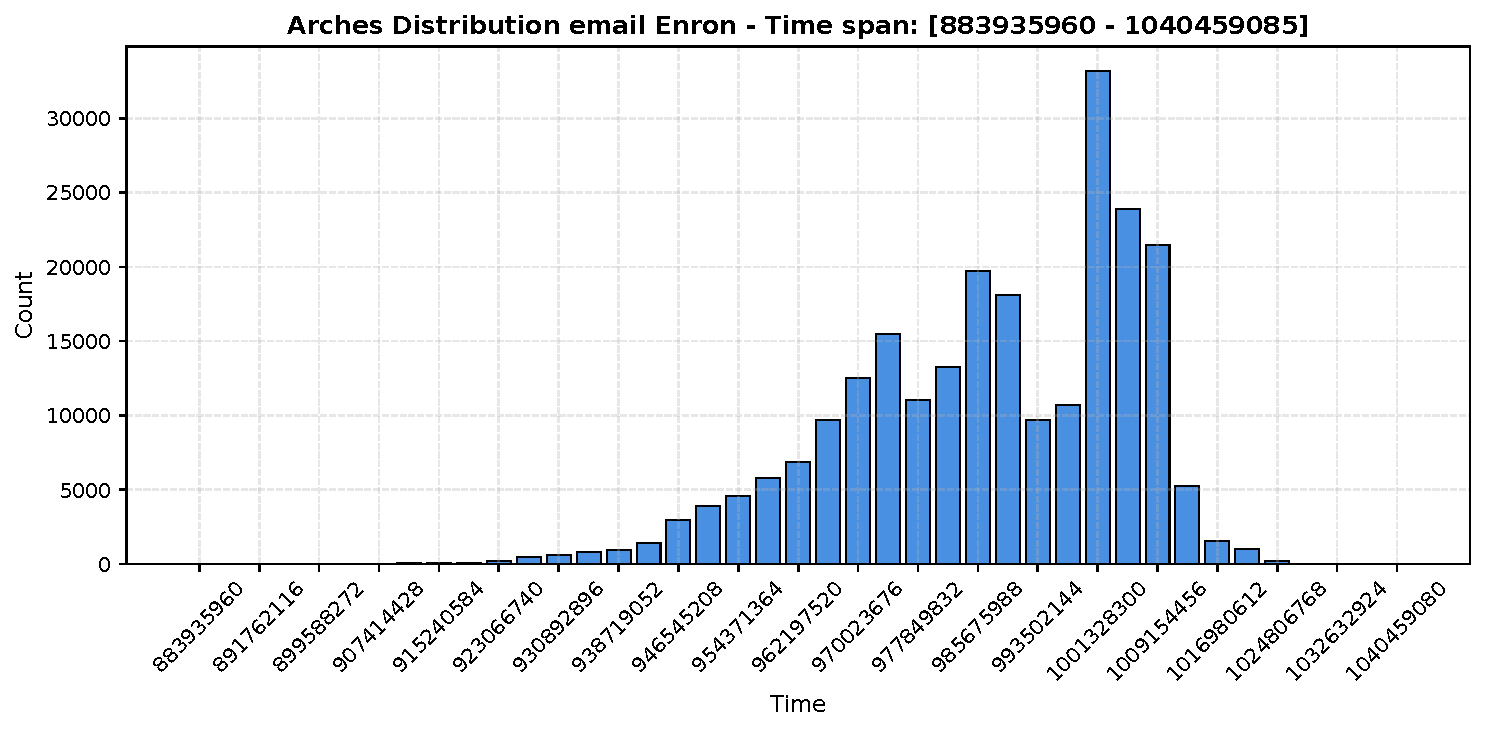
\includegraphics[width=\textwidth]{Immagini/arches_distribution_graph/email_Enron.pdf}
        \vspace{-9mm}
        \caption*{(c) Dataset Email Enron}
    \end{minipage}
    \hfill
    \begin{minipage}{0.48\textwidth}
        \centering
        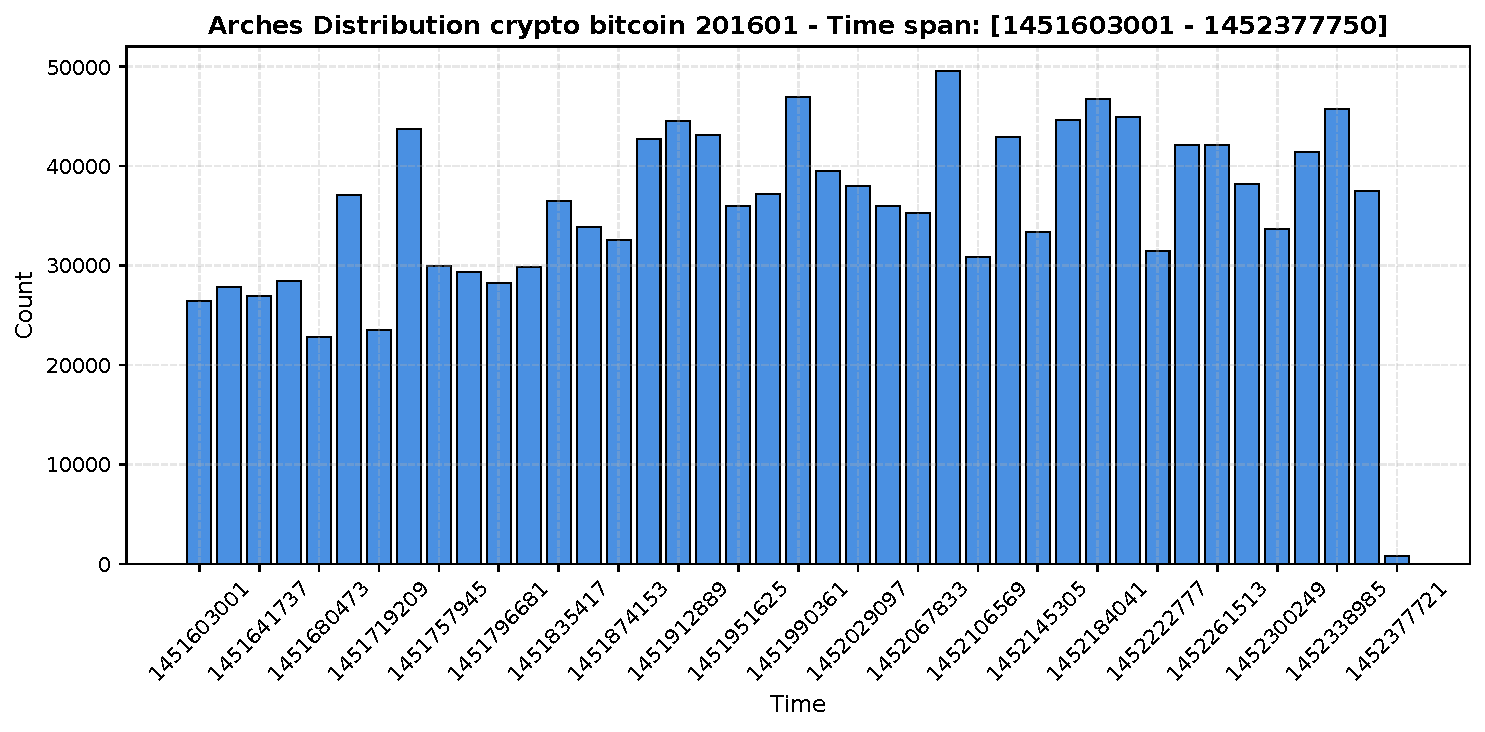
\includegraphics[width=\textwidth]{Immagini/arches_distribution_graph/crypto_bitcoin_201601.pdf}
        \vspace{-9mm}
        \caption*{(d) Dataset Crypto bitcoin}
    \end{minipage}
    \caption{Distribuzione delle frequenze di interazioni nei dataset analizzati.}
    \label{fig:distribuzione_dataset}
\end{figure}
Come si può notare dai profili temporali riportati in figura, i dataset analizzano dinamiche evolutive profondamente differenti tra di loro.
Alcuni di essi sono caratterizzati da periodi di \textit{burst}, ovvero da momenti di picco di attività e da momenti di assenza di iperarchi, mentre altre hanno una distribuzione caratterizzata da un picco di attività ben definito.
Questa forte asimmetria nella distribuzione gioca un ruolo fondamentale nei risultati che ci si può aspettare dall'algoritmo sviluppato.

% 4.4
% Revisione Ready
% Grammatica Ready
% Citazioni Ready

\section{Analisi delle prestazioni computazionali}\label{sec:analisi_delle_presentazioni_computazionali}

In questa sezione vengono presentati e analizzati i riscontri empirici ottenuti dall'esecuzione della soluzione proposta (si veda il Capitolo~\ref{sec:soluzione_proposta}) mettendoli a confronto con delle versioni di confronto (si veda il Capitolo~\ref{sec:varianti_degli_algoritmi_analizzati}) sulle istanze di benchmark precedentemente caratterizzate (si veda il Capitolo~\ref{sec:istanze_di_benchmark_e_caratterizzazione_dei_dati}).
L'obiettivo fondamentale è quello di quantificare l'efficienza e l'efficacia dell'approccio basato sulla finestra temporale a scorrimento, evidenziandone la scalabilità al crescere della dimensionalità del problema.

\subsection{Metriche di valutazione e protocollo di tesi}

Per valutare qualitativamente il comportamento del sistema sono state analizzate le tre metriche precedentemente citate durante la definizione formale del problema (si veda il Capitolo~\ref{sec:definizione_formale}), ovvero:
\begin{itemize}
    \item \textbf{Tempo di esecuzione ($T_{exec}$)}: espresso in secondi, misura il tempo impiegato da parte dell'elaboratore per arrivare al termine dell'esecuzione dell'algoritmo analizzato.
    \item \textbf{Dimensione media dell'Hitting Set ($\overline{|X|}_{\tau}$)}: espresso attraverso il numero di nodi, misura la cardinalità media temporale dell'insieme di copertura calcolato durante l'intero periodo di esecuzione.
    \item \textbf{Numero nodi distinti scelti ($R$)}: espresso attraverso il numero di nodi, rappresenta il volume complessivo di vertici unici accumulati nell'Hitting Set globale al termine del processo (si veda il Capitolo~\ref{sec:definizione_formale}).
\end{itemize}
L'analisi congiunta delle tre metriche permette di mappare accuratamente il trade-off dell'algoritmo proposto tra l'efficienza computazionale del codice e la qualità delle soluzioni generate, offrendo una panoramica completa sulla scalabilità dell'approccio proposto.

\subsection{Aspettative sperimentali e risultati}

Prima di analizzare direttamente i risultati sperimentali, è importante definire un comportamento atteso dell'algoritmo in tutte le sue versioni in modo da poter successivamente confrontare le aspettative con i risultati effettivi.
Poiché l'efficienza della soluzione si basa parzialmente anche sul rapporto tra la dimensione della finestra temporale considerata $(\epsilon)$ e la dimensione dello scorrimento computazionale della stessa $(\delta)$, abbiamo deciso, per ogni dataset analizzato, di testare tre rapporti differenti tra $\epsilon$ e $\delta$ in modo da poter analizzare come cambia il risultato al variare delle loro dimensioni.

\subsubsection*{Contacts high school}

La caratteristica particolare di questo dataset è la distribuzione di arrivo degli iperarchi marcatamente intermittente (si veda Figura~\ref{fig:distribuzione_dataset} a).
Su tale base si può affermare che l'efficacia dell'algoritmo proposto e delle rispettive estensioni può essere garantita solo in base al rapporto che la dimensione della finestra temporale e la dimensione del relativo scorrimento hanno con i picchi e le valli di attività della distribuzione mostrata.
La soluzione proposta riesce dunque a garantire prestazioni ottimali solo a condizione che l'ampiezza della finestra temporale sia sufficiente a intercettare più picchi concorrenti e che il passo di scorrimento sia almeno pari al loro tempo di inter-arrivo.
In pratica l'unico modo affinché l'algoritmo riesca a funzionare con questa distribuzione degli archi in ingresso è selezionando delle dimensioni di $\epsilon$ e $\delta$ in grado di mascherare la presenza dei burst temporali.

\begin{figure}[htbp]
    \centering
    \begin{minipage}{0.32\textwidth}
        \centering
        
\includegraphics[width=\textwidth, trim={0cm 0cm 5cm 0cm}, clip]{Immagini/time_distribution_graphs/contacts_high_school.pdf}
        \vspace{-9mm}
        \caption*{Tempo di esecuzione}
    \end{minipage}
    \hfill
    \begin{minipage}{0.32\textwidth}
        \centering
        
\includegraphics[width=\textwidth, trim={0cm 0cm 5cm 0cm}, clip]{Immagini/size_distribution_graphs/contacts_high_school.pdf}
        \vspace{-9mm}
        \caption*{Dimensione media Hitting Set}
    \end{minipage}
    \hfill
    \begin{minipage}{0.32\textwidth}
        \centering
        
\includegraphics[width=\textwidth, trim={0cm 0cm 5cm 0cm}, clip]{Immagini/reuse_distribution_graphs/contacts_high_school.pdf}
        \vspace{-9mm}
        \caption*{Numero nodi distinti scelti}
    \end{minipage}

    \vspace{2mm}
    % Legenda manuale
    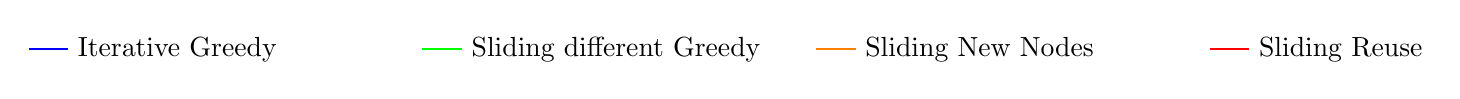
\begin{tikzpicture}
        \draw[blue, thick] (0,0) -- (0.5,0); \node[right] at (0.5,0) {Iterative Greedy};
        \draw[green, thick] (5,0) -- (5.5,0); \node[right] at (5.5,0) {Sliding different Greedy};
        \draw[orange, thick] (10,0) -- (10.5,0); \node[right] at (10.5,0) {Sliding New Nodes};
        \draw[red, thick] (15,0) -- (15.5,0); \node[right] at (15.5,0) {Sliding Reuse};
    \end{tikzpicture}
    
\end{figure}

\subsubsection*{Coauth history}

Come nel grafico precedente, la caratteristica particolare del dataset risiede nella sua distribuzione di arrivo degli iperarchi (si veda Figura~\ref{fig:distribuzione_dataset} b).
La presenza di un picco di nodi verso la fine del periodo temporale studiato non permette di sfruttare la conoscenza acquisita dalle finestre precedenti, limitando le situazioni in cui l'algoritmo riesce a fornire prestazioni migliori.

\begin{figure}[htbp]
    \centering
    \begin{minipage}{0.32\textwidth}
        \centering
        
\includegraphics[width=\textwidth, trim={0cm 0cm 5cm 0cm}, clip]{Immagini/time_distribution_graphs/coauth_history.pdf}
        \vspace{-9mm}
        \caption*{Tempo di esecuzione}
    \end{minipage}
    \hfill
    \begin{minipage}{0.32\textwidth}
        \centering
        
\includegraphics[width=\textwidth, trim={0cm 0cm 5cm 0cm}, clip]{Immagini/size_distribution_graphs/coauth_history.pdf}
        \vspace{-9mm}
        \caption*{Dimensione media Hitting Set}
    \end{minipage}
    \hfill
    \begin{minipage}{0.32\textwidth}
        \centering
        
\includegraphics[width=\textwidth, trim={0cm 0cm 5cm 0cm}, clip]{Immagini/reuse_distribution_graphs/coauth_history.pdf}
        \vspace{-9mm}
        \caption*{Numero nodi distinti scelti}
    \end{minipage}

    \vspace{2mm}
    % Legenda manuale
    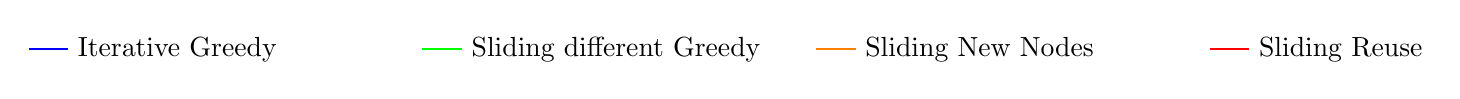
\begin{tikzpicture}
        \draw[blue, thick] (0,0) -- (0.5,0); \node[right] at (0.5,0) {Iterative Greedy};
        \draw[green, thick] (5,0) -- (5.5,0); \node[right] at (5.5,0) {Sliding different Greedy};
        \draw[orange, thick] (10,0) -- (10.5,0); \node[right] at (10.5,0) {Sliding New Nodes};
        \draw[red, thick] (15,0) -- (15.5,0); \node[right] at (15.5,0) {Sliding Reuse};
    \end{tikzpicture}
    
\end{figure}

\subsubsection*{Email Enron}

A differenza dei grafici precedenti, la distribuzione di arrivo degli iperarchi del dataset non sembra poter creare particolari problemi, in quanto la fase di picco è situata a metà del periodo temporale studiato (si veda Figura~\ref{fig:distribuzione_dataset} c).
Tale dataset però risulta essere particolarmente denso (si veda Tabella~\ref{tab:caratteristiche_dataset}), fattore che potrebbe portare a una minore differenza nel numero di nodi distinti scelti $(R)$ e a un buon grado di approssimazione dell'Hitting Set sia da parte degli algoritmi basati su finestra temporale a scorrimento, sia da parte di quelli greedy iterativi.

\begin{figure}[htbp]
    \centering
    \begin{minipage}{0.32\textwidth}
        \centering
        
\includegraphics[width=\textwidth, trim={0cm 0cm 5cm 0cm}, clip]{Immagini/time_distribution_graphs/email_Enron.pdf}
        \vspace{-9mm}
        \caption*{Tempo di esecuzione}
    \end{minipage}
    \hfill
    \begin{minipage}{0.32\textwidth}
        \centering
        
\includegraphics[width=\textwidth, trim={0cm 0cm 5cm 0cm}, clip]{Immagini/size_distribution_graphs/email_Enron.pdf}
        \vspace{-9mm}
        \caption*{Dimensione media Hitting Set}
    \end{minipage}
    \hfill
    \begin{minipage}{0.32\textwidth}
        \centering
        
\includegraphics[width=\textwidth, trim={0cm 0cm 5cm 0cm}, clip]{Immagini/reuse_distribution_graphs/email_Enron.pdf}
        \vspace{-9mm}
        \caption*{Numero nodi distinti scelti}
    \end{minipage}

    \vspace{2mm}
    % Legenda manuale
    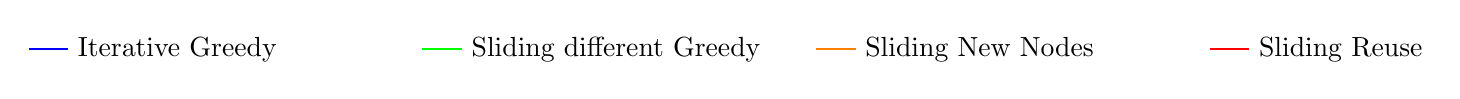
\begin{tikzpicture}
        \draw[blue, thick] (0,0) -- (0.5,0); \node[right] at (0.5,0) {Iterative Greedy};
        \draw[green, thick] (5,0) -- (5.5,0); \node[right] at (5.5,0) {Sliding different Greedy};
        \draw[orange, thick] (10,0) -- (10.5,0); \node[right] at (10.5,0) {Sliding New Nodes};
        \draw[red, thick] (15,0) -- (15.5,0); \node[right] at (15.5,0) {Sliding Reuse};
    \end{tikzpicture}
    
\end{figure}

\subsubsection*{Crypto bitcoin}

L'ultimo dataset risulta essere quello più favorevole dal punto di vista dell'algoritmo da me sviluppato, in quanto presenta una distribuzione di arrivo quasi costante e di una struttura non particolarmente densa.
In presenza di tali condizioni, ci aspettiamo che il nostro algoritmo riesca a sfruttare al meglio il funzionamento della finestra temporale, mentre, a causa della natura sparsa del dataset, ci aspettiamo che gli algoritmi greedy iterativi non riescano a ottenere risultati altrettanto buoni.

\begin{figure}[htbp]
    \centering
    \begin{minipage}{0.32\textwidth}
        \centering
        
\includegraphics[width=\textwidth, trim={0cm 0cm 5cm 0cm}, clip]{Immagini/time_distribution_graphs/crypto_bitcoin_201601.pdf}
        \vspace{-9mm}
        \caption*{Tempo di esecuzione}
    \end{minipage}
    \hfill
    \begin{minipage}{0.32\textwidth}
        \centering
        
\includegraphics[width=\textwidth, trim={0cm 0cm 5cm 0cm}, clip]{Immagini/size_distribution_graphs/crypto_bitcoin_201601.pdf}
        \vspace{-9mm}
        \caption*{Dimensione media Hitting Set}
    \end{minipage}
    \hfill
    \begin{minipage}{0.32\textwidth}
        \centering
        
\includegraphics[width=\textwidth, trim={0cm 0cm 5cm 0cm}, clip]{Immagini/reuse_distribution_graphs/crypto_bitcoin_201601.pdf}
        \vspace{-9mm}
        \caption*{Numero nodi distinti scelti}
    \end{minipage}

    \vspace{2mm}
    % Legenda manuale
    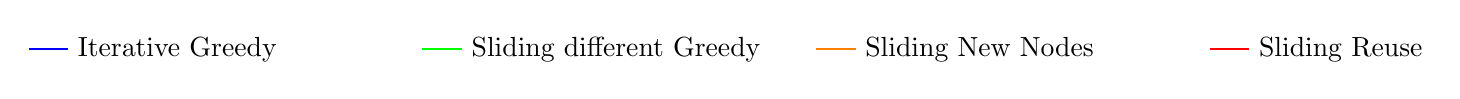
\begin{tikzpicture}
        \draw[blue, thick] (0,0) -- (0.5,0); \node[right] at (0.5,0) {Iterative Greedy};
        \draw[green, thick] (5,0) -- (5.5,0); \node[right] at (5.5,0) {Sliding different Greedy};
        \draw[orange, thick] (10,0) -- (10.5,0); \node[right] at (10.5,0) {Sliding New Nodes};
        \draw[red, thick] (15,0) -- (15.5,0); \node[right] at (15.5,0) {Sliding Reuse};
    \end{tikzpicture}
    
\end{figure}

% 4.5
% Riguardare l'umanità del testo
% Grammatica Ready
% Citazioni Ready

\section{Analisi critica e trade-off}\label{sec:analisi_critica_e_trade_off}

I risultati presentati nella sezione precedente confermano solo parzialmente le aspettative formulate in apertura del capitolo precedente.
L'approccio incrementale non rappresenta un miglioramento universale rispetto alla baseline Iterative Greedy, quanto più un compromesso la cui efficacia dipende fortemente dalla struttura del dataset analizzato.
All'interno della sezione seguente si discutono nello specifico i casi in cui la soluzione proposta ha rispettato le aspettative, i casi in cui le ha disattese, e si tenta di fornire una spiegazione di tali divergenze; viene inoltre analizzato il rapporto che ha la soluzione \texttt{Sliding Reuse} rispetto alle sue versioni \texttt{Sliding different Greedy} e \texttt{Sliding New Nodes}.

\subsection*{Quando l'algoritmo funziona}

I casi d'uso più rappresentativi del comportamento atteso sono stati i dataset Crypto Bitcoin e Email Enron, all'interno dei quali, come predetto correttamente dalle aspettative presentate nel capitolo precedente, gli algoritmi basati su una struttura a finestra temporale a scorrimento hanno osservato dei miglioramenti in fatto di dimensione media dell'Hitting Set $(\overline{|X|}_{\tau})$ e in fatto di numero di nodi distinti scelti $(R)$ rispetto a quelli osservati dall'algoritmo iterativo greedy.
Tali risultati però non sono sempre accompagnati da un analogo vantaggio in termini di tempo di esecuzione, nonostante si possa vedere un leggero vantaggio in termini di tempo di esecuzione all'interno del primo caso di test di Email Enron e di Crypto Bitcoin, per riuscire a definire un miglioramento sostanziale di $T_{exec}$ è necessario aumentare il numero di iperarchi e aumentare il rapporto $\epsilon/\delta$, mantenendo però una distribuzione degli iperarchi costante.
Tale distribuzione di arrivo quasi costante unita alla bassa densità del dataset Crypto Bitcoin ha creato infatti le condizioni ideali affinché l'algoritmo possa esprimersi al meglio.
Risulta inoltre necessario sottolineare come a prescindere dal dataset considerato, la scelta di un rapporto $\epsilon/\delta$ alto ha portato a un miglioramento generale dei risultati, in quanto l'algoritmo è riuscito a sfruttare al meglio, ove possibile, il riutilizzo dei nodi attraverso la finestra temporale a scorrimento.

\subsection*{Quando l'algoritmo non rispetta le aspettative}

Opposti ai casi d'uso presentati precedentemente, i casi d'uso più rappresentativi di un comportamento inatteso sono stati i dataset Coauth history e Contacts high school.
Come previsto all'interno del capitolo precedente, a causa della non stazionarietà nella distribuzione degli arrivi degli iperarchi, in entrambi i casi si è potuto notare come l'aumento nel tempo di esecuzione totale $(T_{exec})$ non sia stato corrisposto da una diminuzione significativa e apprezzabile dal punto di vista della dimensione media della soluzione $(\overline{|X|}_{\tau})$ e del numero di nodi distinti scelti $(R)$.
Tali risultati sono motivati dal fatto che, quando le interazioni si concentrano in burst isolati o in un singolo picco terminale, la memoria storica costruita dall'algoritmo non ha modo di essere sfruttata prima che la finestra si sposti oltre, vanificando l'investimento computazionale fatto per mantenerla.
Va precisato che l'effetto non risulta completamente identico nei due dataset, su Coauth history il margine di miglioramento risulta nullo o negativo in quasi tutte le configurazioni testate, mentre nel caso di Contacts high school la soluzione mantiene un vantaggio minimo ma non sempre nullo, segno che la sola intermittenza della distribuzione non è sufficiente ad annullare del tutto il beneficio del riuso, ma ne riduce significativamente l'entità rispetto ai casi favorevoli discussi in precedenza.

\subsection*{Confronto tra le varianti algoritmiche}

I risultati ci consentono inoltre di valutare quanto le singole scelte progettuali (si veda il Capitolo~\ref{sec:varianti_degli_algoritmi_analizzati}) abbiano effettivamente impattato sul comportamento del sistema finale.
L'analisi delle tre varianti mostra infatti che non tutte le modifiche progettuali hanno prodotto un cambiamento radicale e che l'effetto di ciascuna dipende dalla componente dell'algoritmo che viene alterata.
La variante \texttt{Sliding different Greedy}, che adotta una selezione randomica dell'iperarco di riferimento invece che a cardinalità minima, mostra un comportamento discontinuo sul tempo di esecuzione a causa della sua componente randomica.
Nonostante in alcuni casi di test tale algoritmo fornisca soluzioni leggermente migliori rispetto a quelle viste nell'algoritmo Sliding Reuse, i risultati sono quasi completamente comparabili, se non addirittura in media leggermente peggiori.
Va peraltro riconosciuto che questa variante minima è causata dalla variazione minima che è stata applicata all'interno della stessa euristica hyperedge-oriented; un test più probante avrebbe richiesto un'euristica vertex-oriented strutturalmente distinta come quella descritta da Johnson~\cite{johnson1974} all'interno del capitolo riguardo allo stato dell'arte (si veda il Capitolo~\ref{sec:minimum_hitting_set_in_ambito_statico}).
La variante \texttt{Sliding New Node}, che inverte la priorità della funzione ReuseGreedyHittingSet preferendo nodi privi di storico, produce invece un effetto netto e coerente con l'ipotesi di progettazione.
Come si può notare all'interno delle soluzioni mostrate in tutti i dataset, essa presenta un numero di nodi distinti scelti $(R)$ peggiore, o al più comparabile, rispetto a quello denotato all'interno di Sliding Reuse, e un generale aumento nel tempo di esecuzione totale $(T_{exec})$.
In conclusione, il confronto tra varianti suggerisce che la componente realmente determinante del sistema non sia tanto l'algoritmo greedy di base, quanto piuttosto la politica di priorità nel riuso dei nodi, la cui sola inversione è sufficiente a vanificare gran parte del beneficio in $R$ ottenuto dalla soluzione proposta.

\subsection*{Il costo computazionale come contropartita sistematica}

Un risultato trasversale a tutti i dataset analizzati è che il tempo di esecuzione di \texttt{Sliding Reuse} risulta quasi sempre superiore a quello di Iterative Greedy, indipendentemente dalla qualità della soluzione ottenuta.
Tale risultato, in apparenza in contrasto con l'obiettivo dichiarato in fase di progettazione (si veda il Capitolo~\ref{sec:soluzione_proposta}), trova spiegazione nell'analisi di complessità (si veda il  Capitolo~\ref{sec:considerazioni_sulla_complessità}).
All'interno della soluzione la funzione \texttt{Cleanup}, che nel caso pessimo richiede l'esecuzione della funzione \texttt{ReuseGreedyHittingSet} sull'intera porzione di finestra ancora scoperta, introduce dei costi computazionali non trascurabili rispetto a quelli che si trovano all'interno di un algoritmo greedy puro, privo di strutture ausiliarie da mantenere e consultare a ogni passo.
Il prezzo pagato per ottenere un minor turnover dei nodi nel tempo si traduce dunque in un aumento del lavoro richiesto per ciascun singolo aggiornamento.

\subsection*{Contesti d'uso e limiti dell'approccio}

Analizzando l'insieme delle osservazioni precedenti emergono alcune situazioni in cui l'algoritmo riesce a sfruttare appieno il potenziale della finestra temporale a scorrimento.
La soluzione proposta risulta particolarmente vantaggiosa in tutti quei casi in cui la distribuzione di arrivo degli iperarchi può essere considerata relativamente uniforme nel tempo e priva di crescite esponenziali capaci di concentrare la maggior parte degli eventi in una porzione ristretta della finestra di osservazione.
Al contrario, l'algoritmo risulta poco indicato, o nei casi peggiori controproducente, in presenza di forte burstiness o di picchi concentrati di attività, come osservato nel dataset Coauth history, e in tutti i contesti nei quali il vincolo principale è la latenza di aggiornamento piuttosto che il numero di nodi distinti coinvolti nel tempo.
In tali casi il costo aggiuntivo della gestione dello storico non viene ripagato da un miglioramento della qualità della soluzione, rendendo l'algoritmo iterativo greedy una scelta preferibile nonostante la sua natura non incrementale.
Va infine osservato come il trade-off identificato non sia univoco nemmeno all'interno dello stesso dataset, ma dipenda anche dal rapporto tra l'ampiezza della finestra $\epsilon$ e il passo di scorrimento $\delta$.
Quando il rapporto tra le due tende a infinito, ovvero quando si considerano finestre temporali più ampie e un minor spostamento di tale finestra, la soluzione implementa attraverso l'utilizzo della finestra temporale a scorrimento risulta migliore a causa della maggiore opportunità di riutilizzo dei nodi e del minore ricalcolo necessario, mentre quando il rapporto tende a uno o a un valore minore di uno, l'utilizzo della finestra temporale a scorrimento aggiunge solamente dei costi computazionali che non è in grado di coprire.
La scelta dei parametri $\epsilon$ e $\delta$ rimane quindi, anche alla luce dei risultati sperimentali, un compromesso da calibrare sul contesto applicativo specifico, piuttosto che un valore universalmente ottimale.

% subchaprters
%% Controllato, teoricamente dovrebbe andare bene sia a lunghezza che a grammatica

\section{Context}\label{sec:context}

The increasing availability of relational data that has been studied in recent years has led to a growing interest in the study of data structures capable of representing complex interactions between entities.
In the literature, such type of relationship were originally managed by means of \textit{graphs}, which are mathematical structures used to model one-to-one relations between objects.
However, many real-world scenarios find this representation too restrictive, when considering interactions between more than just two entities.
\newline
Several real-life scenarios are by default not representable as graphs.
Some examples include conversations between multiple people, usually found online in forums, chat or more generally in social media, while others include the interactions between multiple objects or entities, such as those involved in a bank transaction.
In these types of contexts, the loss of information when representing these interactions as graphs is unavoidable.
\newline
In order to be able to manage this type of data relationship, the concept of \textit{hypergraph} was introduced.
An hypergraph is a generalization of a graph, characterized by the introduction of many-to-many relationships between entities, which are called \textit{hyperedges}.
This type of data structure is particularly useful when the goal is to represent complex interations without losing sensitive information, as it is the case with graphs.
\newline
In real life scenarios, the interactions between entities are not static, but they evolve over time.
New interactions are created, while others tend to disappear, this brings to a complex dynamic system that brings a theoretically static data structure to evolve over time.
This type of challenge makes the management of this temporal evolution a necessity, in order to be able to represent the data always in an accurate way.
\newline
The analysis of large dynamic structures also introduces important computational problems.
In particular, it is often necessary to continuously update the information of interest without being able to recalculate the entire solution from scratch each time.
Consequently, the study of efficient techniques for the maintenance of combinatorial properties and structures in dynamic and temporal environments assumes a central role.